\documentclass[12pt, donotrepeattitle, jou]{apa6}
\usepackage[utf8]{inputenc}
\usepackage[spanish]{babel}
\usepackage{graphicx}
\usepackage[style=apa,sortcites=true,sorting=nyt,backend=biber]{biblatex}
\title{Identificando el riesgo de suicidio a través de una red neuronal capsular usando datos de Facebook}
\shorttitle{Suicidio, inteligencia artificial y Facebook}
\author{Juan D. Angarita - Sharol G. Torres}
\affiliation{Universidad Popular del Cesar}
\addbibresource{bibliography.bib}
\abstract{Una de las principales causas de muerte que ha tenido un aumento dramático en los últimos años en Colombia es el suicidio. Esta situación tiene un componente inherente que lo hace difícil de prevenir: es muy complejo identificar a las personas en riesgo. En el presente estudio mostraremos cómo (usando un enfoque tecnológico) es posible identificar con un porcentaje de acierto elevado a las personas en riesgo. Utilizando la información pública de Facebook de personas que se han suicidado, hemos entrenado una red neuronal capsular para que pueda llevar a cabo dicha labor. Elementos tales cómo: cambios en la preferencia de colores, horas de publicación recurrente y contenido textual de sus perfiles, han pobrado estar relacionados con la problemática. }

\keywords{suicidio, facebook, redes neuronales capsulares, análisis de sentimientos}

\begin{document}
    \maketitle
    \section{Introducción}
    A día de hoy, identificar de forma masiva los factores, señales y patrones que dan origen al pensamiento suicida o la
    consumación del mismo sigue siendo una tarea que parece superar todos nuestros esfuerzos. Evidentemente, la conducta suicida representa un desafío complejo para las ciencias humanas, en el que las causas que desencadenan la crisis se interrelacionan de tal forma, que detectarlas puede ser un proceso muy largo. Como flagelo social, este ha sido foco investigativo en diversas disciplinas, cada una encarando el problema de una forma distinta y, sin embargo, los resultados siguen siendo poco aplicables. 
    
    Entre tanto, según estadísticas del \textcite{MedicinaLegal}, la autoeliminación ha venido escalando entre las principales causas de muerte por factores externos en Colombia, siendo la población más afectada sujetos entre 20 y 34 años.
    
    Considerando que la población más afectada por esta problemática es también la de mayor acceso a redes sociales \parencite{Facebook}, y dado el aumento de la tendencia a publicar contenido sobre su estado de ánimo en perfiles públicos de Internet, podemos anticipar que explorar estos espacios en busca de elementos comunes entre ellos, puede conducir a la identificación de patrones ignorados hasta ahora, lo que a su vez aumentaría la detección temprana de riesgo potencial e ideación e intento suicida.
    
    Elementos tales cómo: cambios en la preferencia de colores\parencite{Carruthers2010}, aumento de actividad nocturna \parencite{Season} y un discurso marcado por algunas palabras clave \parencite{TextAnalysis}, han probado estar relacionados con la depresión y aparición de ideas suicidas y las redes sociales son sitios propicios para rastrear dichos elementos.

    Uno de los elementos limitantes en la lucha contra el suicidio es la falta de detección temprana, es por ello que este estudio se basará en el perfilamiento de las señales y todas las variables que inciden en la consumación del suicidio y sus manifestaciones previas.
    
    Se sostiene que la funcionalidad de las alertas primarias debe tomarse como señales que conducirán a la necesaria detección temprana, lo que implica necesariamente el reconocimiento del suicidio como proceso en el que existen diversos factores intervinientes, que finalmente llevan al sujeto a la decisón de consumar el acto. Por lo que se considera fundamental tener conocimiento sobre el proceso y los eventos que ocurren anteriormmente a que la persona llegue a esta decisión fatal. Dichos eventos son la ideación suicida y el intento de suicidio \parencite{SANCHEZ2010}.
    
    Lamentablemente, la detección temprana sigue siendo una deuda pendiente de la investigación con la sociedad. Sin embargo, tomando como base el más reciente avance de la inteligencia artificial y usando como catalizador un algoritmo de redes neuronales capsulares, analizaremos la producción textual, visual, los patrones de actividad, las preferencias en los cambios de colores y otras variables recolectadas en perfiles públicos de suicidas en facebook; con el objetivo de poder entrenar eficientemente un modelo que nos permita usando la misma información proveniente de perfiles comunes, identificar aquellas personas que están dando señales de estar ante un riesgo inminente.
    
    Confiamos en que de la integración de algoritmos de inteligencia artificial y conocimientos psicológicos, vendrá la próxima revolución de nuestro campo. Existen numerosas variables cuantitativas que podrían darnos muestras claras de patrones que a día de hoy siguen velados para la investigación tradicional, puesto que, nuestra capacidad de detección de patrones y procesamiento numérico palidece ante la sofisticación actual de las máquinas.

    \subsection{Paradigma de redes neuronales actual}
    En los últimos años, las investigaciones en el campo de inteligencia artificial (en lo que se refiere al aprendizaje profundo) se centraron en cómo aumentar la profundidad de una red, agregando más capas para lograr un mayor grado de abstracción (comenzando desde las primeras capas convolucionales capaces de extraer formas pequeñas, ángulos o intensidad de color, vamos paso a paso combinando características simples en diseños cada vez más complejos)\parencite{Capsules}.
    
    Para hacer esto, tenemos que mantener bajo control el número de parámetros (y los tiempos computacionales) usamos un operador, común en todas las redes profundas, osea un pooling que nos permite que reduzca el número de parámetros reduciendo progresivamente el componente espacial seleccionando los valores más altos pero perdiendo la información espacial relacionada con las características extraídas\parencite{Capsules2}.
    
    \subsection{Redes neuronales capsulares}
    Por lo tanto, la investigación sobre la arquitectura de las redes neuronales se centra progresivamente en el objetivo de aprender a generalizar mejor en lugar de proporcionar datos cada vez más procesados \parencite{Capsules3}. Se realizó un primer paso con las redes neuronales capsulares, donde nuestro objetivo es obtener una Equivariancia (invarianza de las rototraslaciones) que reemplace al operador de pooling con una nueva estructura denominada: Dynamic Routing.
    
    Una cápsula es un grupo de neuronas. La actividad de un vector de una cápsula representa los parámetros de instanciación cuando un objeto (o parte de él) viene detectado por la red. La longitud de este vector representa la probabilidad de existencia de la clase dada, mientras que la orientación del vector codifica información espacial (por ejemplo, rotaciones y traducciones) dentro de una matriz de posa.
    
    \subsection{Arquitectura redes neuronales capsulares}
    La principal diferencia en las redes capsulares, por lo tanto, consiste en una arquitectura no profunda.
    
    \begin{center}
        \begin{minipage}{0.6\linewidth}
            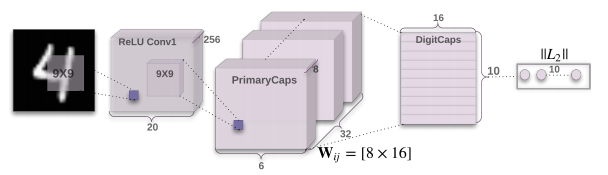
\includegraphics[width=\linewidth]{images/capsules}
            \captionof{figure}{Esquema básico red neuronal capsular}
        \end{minipage}
    \end{center}

    La primera capa convolucional (256 kernels, 9x9,stride igual a uno, activación ReLu)
    En la primera capa convolucional vamos a convertir la intensidad de los píxeles en características de bajo nivel, no nos importa mantener la posición espacial relativa; de hecho, queremos utilizar todas esas propiedades importantes par acompartir parámetros útiles para reducir los tiempos computacionales.

    PrimaryCaps consiste en dos capas ocultas: La primera capa corresponde al proceso de rendering el cual lo hemos descrito antes. La segunda capa, por el contrario, es convolucional (32 cápsulas 8 dimensionales) donde cada cápsula representa una característica extraída, por lo tanto, a través de una convolución de 9x9 kernels y un ritmo igual a dos. El output de PrimaryCaps consiste por lo tanto, en cápsulas de 32x6x6 8 dimensiones.

    La última capa por reproducir en forma vectorial h FC-Layer, es decir, vamos a reducir el número de neuronas (en este caso de cápsulas) para obtener una para cada clase del objetivo\parencite{Capsules4}.

    \begin{itemize}
        \item Reemplazar las neuronas con las cápsulas.
        \item Reemplazar el max-pooling con dynamic routing.
        \item Arquitectura no profunda.
    \end{itemize}

    \section{Métodos}
    \subsection{Participantes}
    Para hacer la identificación de los patrones relacionados con la conducta suicida, utilizamos 20 perfiles de Facebook con contenidos públicos de personas que cometieron, intentaron cometer o han estado en situación de riesgo frente al suicidio. El promedio de edad de los sujetos referenciados en los perfiles es de 21 años ($\sigma = 4.5$), 11 hombres y 9 mujeres.
    
    \subsection{Materiales}
    Para la recolección masiva de la información se utilizó un ``scrapper'', tomando como base el framework Selenium, la información fue almacenada en bases de datos usando el motor Postresql y los algoritmos de inteligencia artificial se apoyaron en los servicios cognitivos de Microsoft, Amazon web services y Tensorflow. Todos los algoritmos mencionados anteriormente fueron programados en el lenguaje Python.
    
    \subsection{Procedimiento}
    La recolección masiva de la información se hizo de manera autónoma y recursiva por el ``scrapper'' que fue programado para escanear todos los perfiles y almacenar en la base de datos la información general, fotos subidas, publicaciones compartidas, estados escritos, reacciones, lista de amigos e intereses.
    
    Posteriormente, con toda la información recolectada y almacenada en la base de datos se procedió a utilizar una red neuronal capsular para examinar todas las publicaciones e imágenes compartidas con el propósito de identificar los elementos en cada imagen, su esquema de colores y la presencia de elementos textuales.
    
    \begin{center}
        \begin{minipage}{0.6\linewidth}
            
\includegraphics[width=\linewidth]{images/1}
            \captionof{figure}{Una de las imágenes compartidas}
        \end{minipage}
    \end{center}
    
    La figura 1 muestra una de las imágenes compartidas en el perfil de uno de los suicidas. Para dicha imagen el algoritmo extrajo el texto para su posterior análisis y generó la siguiente tabla de colores:
    \begin{itemize}
        \item Color 1: Plateado(196, 196, 196). Pixeles: 153398. Porcentaje: 86.75\%
        \item Color 2: Gris oscuro(111, 110, 116). Pixeles: 16589. Porcentaje: 9.38\%
        \item Color 3: Negro(9, 9, 11). Pixeles: 6833. Porcentaje: 3.86\%
    \end{itemize}

    Cuando todas las imágenes se procesaron, se prosiguió a tomar el texto escrito en cada imagen, publicación y elemento compartido para evaluarlo a través de un analizador de sentimientos. El enfoque utilizado fue dividir los textos en frases y examinar una por una en los servicios cognitivos de Microsoft. Una vez obtenido el puntaje de cada frase (entre 0 y 1), se examinó el texto completo y se compararon los resultados para evitar que la presencia de algunas frases positivas alteraran el puntaje de una publicación mayoritariamente negativa.

    \section{Resultados}
    De entre los perfiles que fueron sometidos al análisis, se encontraron que 5 de ellos no contenían la cantidad mínima de publicaciones en el último mes antes de la fecha de suicidio, por lo tanto, fueron descartados para evitar que dicha limitación afectara los resultados finales. Esta es una dificultad que responde a dos causas principales: la primera de ellas es la política de privacidad de datos de Facebook, que será discutida más adelante y la segunda es la tendencia que tienen algunas personas a alejarse del ojo público semanas antes de cometer el acto \parencite{SuicidalB}.
    
    
    Por otro lado, al hacer el análisis estadístico de los valores arrojados por los perfiles restantes, la inteligencia artificial nos permitió observar tres patrones importantes que en el pasado han probado estar relacionados con la ideación suicida y el acto en sí mismo. En primer lugar, la figura 2 nos muestra los porcentajes de representatividad que tuvieron los colores en las imágenes compartidas por los sujetos en el último mes anterior a su muerte.
    
    \begin{center}
        \begin{minipage}{0.8\linewidth}
            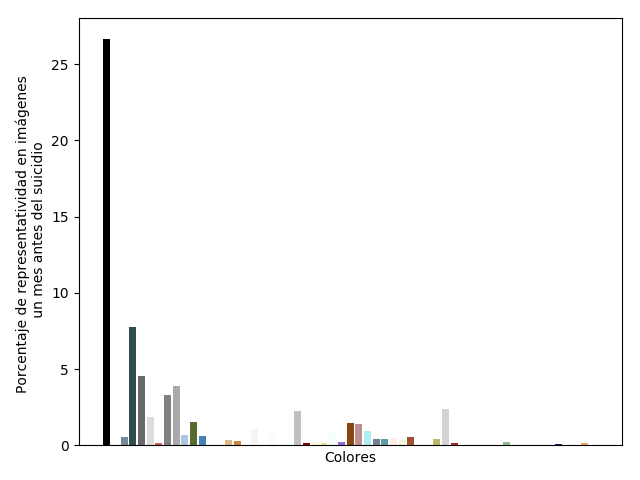
\includegraphics[width=\linewidth]{images/colors_global}
            \captionof{figure}{Imagen acumulativa de los porcentajes de representatividad de los perfiles acumulados}
        \end{minipage}
    \end{center}

    La figura nos muestra que existe una preferencia marcada por los sujetos en riesgo de suicidio hacia cierta gama de colores. Los colores más sobresalientes son el negro, las diferentes tonalidades de grises y algunos otros colores como el verde, rojo y café en sus tonos más oscuros. Estos datos coinciden con el estudio llevado a cabo por \textcite{Carruthers2010}, cuyos datos demostraban que las personas en estado de depresión o con problemas de ansiedad tienen una tendencia a preferir los colores en la escala de grises y los tonos oscuros de entre los 38 colores estudiados.
    
    \begin{center}
        \begin{minipage}{0.3\linewidth}
            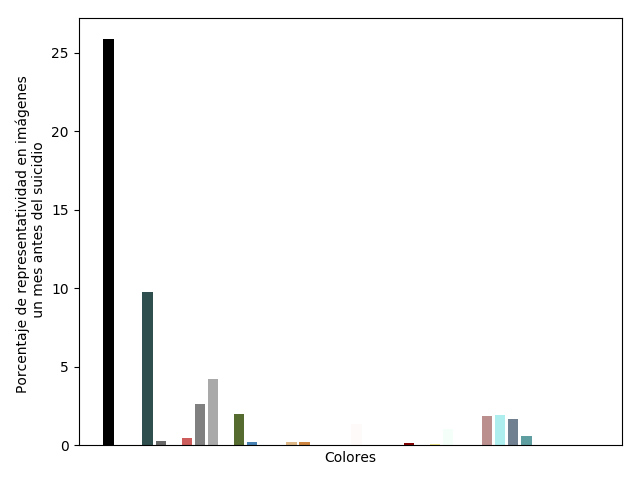
\includegraphics[width=\linewidth]{images/colors_angie}
            \captionof{figure}{Preferencia de colores - Sujeto 1}
        \end{minipage}
        \begin{minipage}{0.3\linewidth}
            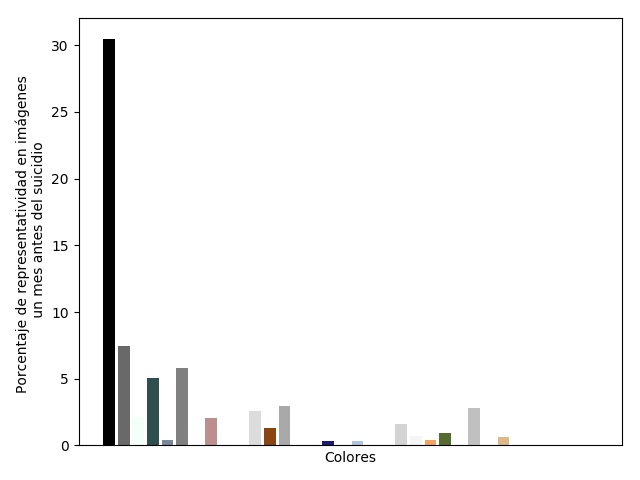
\includegraphics[width=\linewidth]{images/colors_juan}
            \captionof{figure}{Preferencia de colores - Sujeto 4}
        \end{minipage}
        \begin{minipage}{0.3\linewidth}
            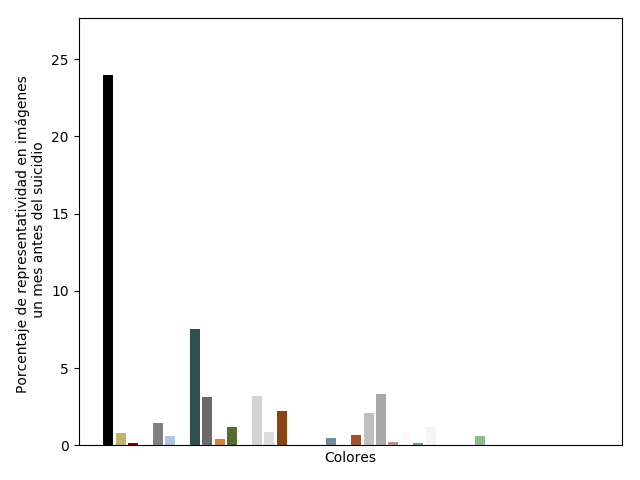
\includegraphics[width=\linewidth]{images/colors_gabriel}
            \captionof{figure}{Preferencia de colores - Sujeto 5}
        \end{minipage}
    \end{center}
    
    Las figuras 3, 4 y 5 nos muestran el caso puntual de tres de los sujetos con mayor número de publicación de imágenes y cuya tendencia es muy notable. Cabe aclarar, para cerrar este patrón, que el porcentaje desbordado del color negro puede estar relacionado con el hecho de que muchas de las imágenes que contenían textos, estaban escritas con fuentes de dicho color.
    
    El segundo patrón observado, relaciona el análisis sentimental hecho al contenido textual de las publicaciones, el texto encontrado en las imágenes y el texto compartido proveniente de publicaciones de terceros que los sujetos publicaban en sus perfiles \parencite{Twitter}.
    
    En este caso en particular pudimos observar que es posible que existan dos patrones relacionados al tono de los textos y que eso implicaría que habría que entrenar las herramientas para poder generar alertas adecuadas para las dos situaciones \parencite{TextAnalysis}. Uno de ellos hace referencia a aquellos sujetos cuya disminución en el puntaje se presenta de forma gradual, mientras que parecen existir algunos sujetos cuyo deterioro es muy rápido.
    
    \begin{center}
        \begin{minipage}{0.45\linewidth}
            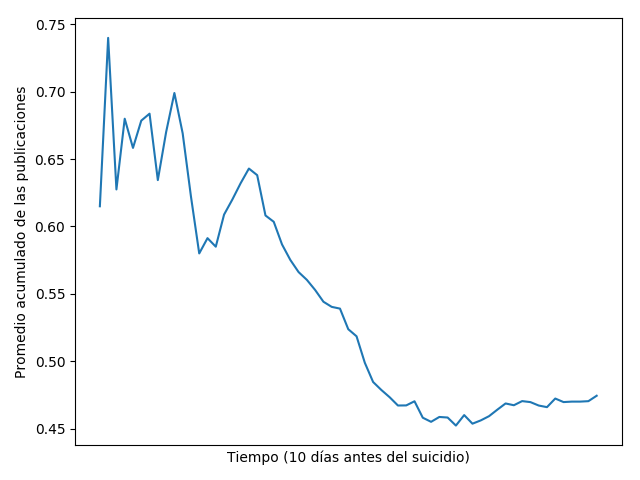
\includegraphics[width=\linewidth]{images/score_angie}
            \captionof{figure}{Análisis textual - Sujeto 7}
        \end{minipage}
        \begin{minipage}{0.45\linewidth}
            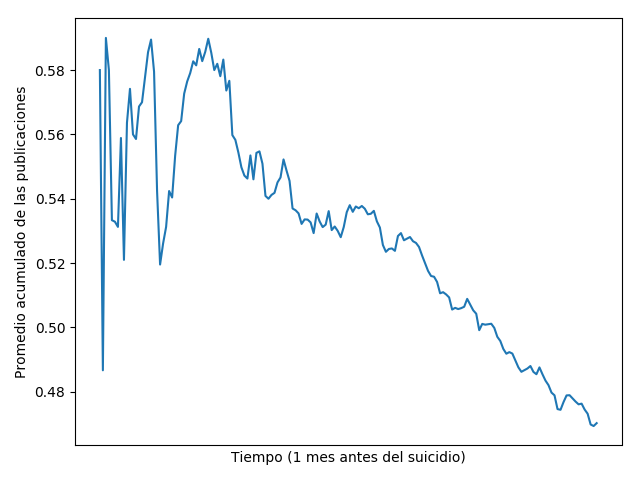
\includegraphics[width=\linewidth]{images/score_juan}
            \captionof{figure}{Análisis textual - Sujeto 13}
        \end{minipage}
    \end{center}
    
    Como podemos observar en las figuras 6 y 7, la escala de tiempo del sujeto 7 es de tan sólo diez días, mientras que el sujeto 13 tiene una escala de un mes. Esto se debe a que la inteligencia artificial hacía el corte de datos cuando encontraba que el sujeto regresaba a los valores promedio. La figura 8, por otro lado, muestra los dos sujetos en una línea de tiempo de 50 días con el objetivo de que se aprecie con mayor claridad la aparición y diferenciación de los dos patrones mencionados anteriormente.
    
    \begin{center}
        \begin{minipage}{0.65\linewidth}
            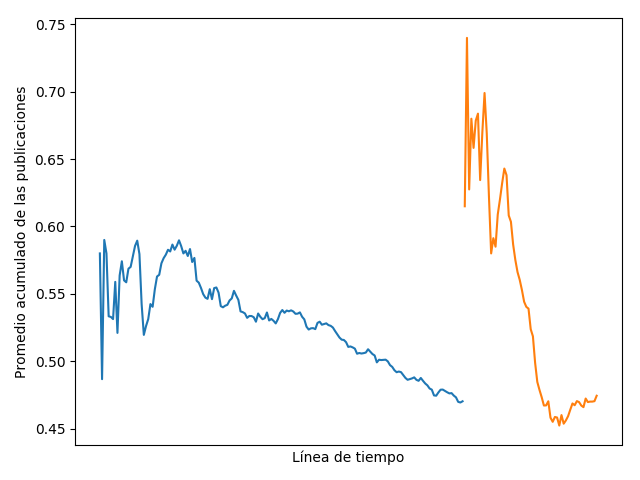
\includegraphics[width=\linewidth]{images/mix}
            \captionof{figure}{Análisis textual - Sujetos 7 y 13}
        \end{minipage}
    \end{center}

    Un posible patrón interesante que nos gustaría medir en el futuro y para el que necesitaríamos un número mayor de datos es el que relaciona los dos patrones anteriores con el estado de ánimo general de los sujetos. A priori, parece observarse que aquellas personas cuyos estados de ánimo está por debajo del promedio en condiciones normales, suelen tener la disminución gradual, mientras que aquellas personas que mantienen un estado de ánimo en la media o superior paracen ser más suceptibles a las disminuciones repentinas.
    
    El último patrón está relacionado con la aparición o aumento de la actividad nocturna por parte de los sujetos antes del suicidio. Puntualmente, hemos medido la actividad realizada entre las 12 de la noche y las 6 de la mañana. Esta franja ha sido identificada por múltiples estudios como la más común para la ejecución del suicidio y la que mayor aumento en los niveles de actividad presenta en los días anteriores al acto. \parencite{Season} \parencite{Littlewoode012113} \parencite{Sleeping} \parencite{PERLIS2016101}.
    
    En promedio, la actividad aumento entre un 40 y un 60 \% ($\sigma = 12.5\%$) durante los días previos a la consumación del suicidio.
    
    \begin{center}
        \begin{minipage}{0.39\linewidth}
            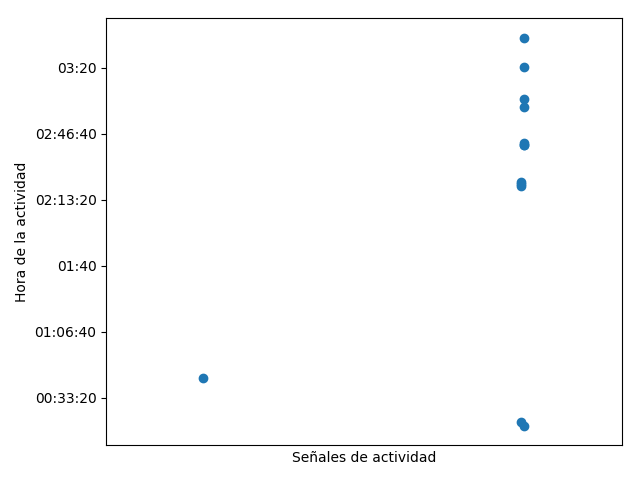
\includegraphics[width=\linewidth]{images/time_angie}
            \captionof{figure}{Act. nocturna - Sujeto 14}
        \end{minipage}
        \begin{minipage}{0.39\linewidth}
            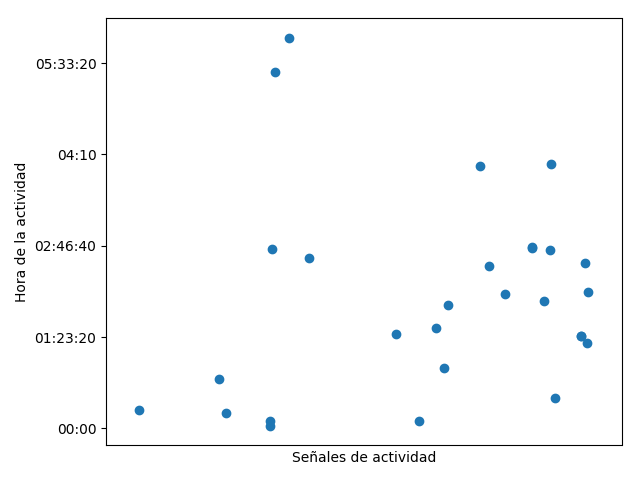
\includegraphics[width=\linewidth]{images/time_juan}
            \captionof{figure}{Act. nocturna - Sujeto 9}
        \end{minipage}
    \end{center}
    
    La figura 9 nos muestra la aparición repentina de actividad nocturna en el sujeto 14, cuya actividad nocturna previa era prácticamente nula. Personas con un patrón de actividad nocturna alto (figura 10), también vieron incrementado el nivel de dicha actividad, los días antes del suicidio.

    \section{Discusión}
    Como hemos podido observar, a pesar de la diversidad demográfica de los perfiles de los sujetos utilizados durante esta investigación, existen algunos patrones generalizados que son identificables de forma masiva \parencite{Twitter}, y que nos permitirían ante una eventual creación de un instrumento más robusto poder reaccionar a tiempo ante un riesgo potencial de suicidio.
    
    Al analizar el flujo de información provista por los mismos sujetos en sus redes sociales, se encontraron elementos que ven aumentada su frecuencia de aparición temporalmente durante momentos de crisis, episodios depresivos y demás situaciones relacionadas al suicidio. Lamentablemente, debido a las configuraciones de privacidad establecidas en la mayor parte de los perfiles de Facebook, el entrenamiento que hemos podido hacer sigue teniendo sus limitaciones. Tal vez, redes sociales con otras tendencias de privacidad como Twitter puedan arrojar datos que permitan potenciar el entrenamiento de nuestro algoritmo.
    
    Por otro lado, es importante recalcar la trascendencia que tuvo en nuestra investigación la implementación de las redes neuronales capsulares, sobretodo a la hora de clasificar y procesar las imágenes. Comparadas con sus predecesoras las redes neuronales convolucionales, este nuevo paradigma de inteligencia artificial ha probado ser sumamente efectivo para la investigación de elementos tan complejos como los patrones de comportamiento humano. Si bien, son más lentas y complejas de calibrar, una vez que se ha llegado al punto de entrenamiento ideal, los datos se procesan de una manera más coherente y cercana a como lo hace nuestro cerebro \parencite{Convolutional}.
    
    Animamos a la comunidad a partir de nuestros resultados y ampliar el espectro del instrumento investigativo, buscando patrones que puedan haber sido ignorados por nuestro enfoque y que finalmente se alcance un modelo más estructurado y eficiente que nos permita desarrollar mecanismos de acción temprana ante el flagelo del suicidio.
    \printbibliography
    
\end{document}